%% content.tex
%%

%% ===========================
\chapter{Umsetzung}
%% ===========================

%% ===========================
\section{Gewichtung der Zeit}
%% ===========================

Der Ansatz zur Umsetzung der Gewichtung der Zeit wird anhand der Abbildung \ref{fig:umsetzung:gewichtungderzeit} erklärt. Die Abbildung zeigt ein Koordinatensystem welches die Gewichtung einzelner Zeitpunkte aufzeigt. Die x-Achse stellt den zeitlichen Verlauf dar. Während die y-Achse die Gewichtung darstellt. $t_{start}$ markiert den Startzeitpunkt, wohingegen $t_{end}$ den Endzeitpunkt angibt. Mithilfe von $t_1$ und $t_2$ werden Zeitspannen festgelegt, die differenziert gewichtet werden sollen. 

\begin{equation}
f_1 = \frac{1}{t_1 - t_{start}}
\end{equation}
\begin{equation}
f_2 = \frac{1}{t_{end} - t_2}
\end{equation}

...

\begin{figure}[htbp]
\begin{center}
\begin{tikzpicture}[domain=-1:2] \draw[very thin,color=gray] (0,0); 
\draw[->] (0,0) -- (12.3,0) node[right] {Zeit}; 
\draw[->] (0,0) -- (0,4.2) node[above] {Faktor Gewichtung}; 
\draw[color=black]  (0.2,3) -- (-0.2,3)   node[left] {100\%};
\draw[color=black]  (0.2,1.5) -- (-0.2,1.5)   node[left] {50\%};  
\draw[dashed][color=black]  (5,0.5) -- (5,3.5); 
\draw[dashed][color=black]  (9,0.5) -- (9,3.5);

\draw[color=black]  (0,0) -- (0,0)   node[below] {$t_{start}$}; 
\draw[color=black]  (5,0.1) -- (5,-0.1)   node[below] {$t_1$}; 
\draw[color=black]  (9,0.1) -- (9,-0.1)   node[below] {$t_2$};
\draw[color=black]  (12,0.1) -- (12,-0.1)   node[below] {$t_{end}$};   
 
\draw[color=black]  (0,0) -- (5,3)   node[right] {}; 
\draw[color=black]  (5,3) -- (9,3)   node[right] {}; 
\draw[color=black]  (9,3) -- (12,0)   node[right] {};  

\end{tikzpicture} 
\end{center}
\caption{Gewichtung der Zeit}
\label{fig:umsetzung:gewichtungderzeit}
\end{figure}

%% ===========================
\section{Klassen der Logik}
%% ===========================

\begin{figure}[htbp]
\begin{center}
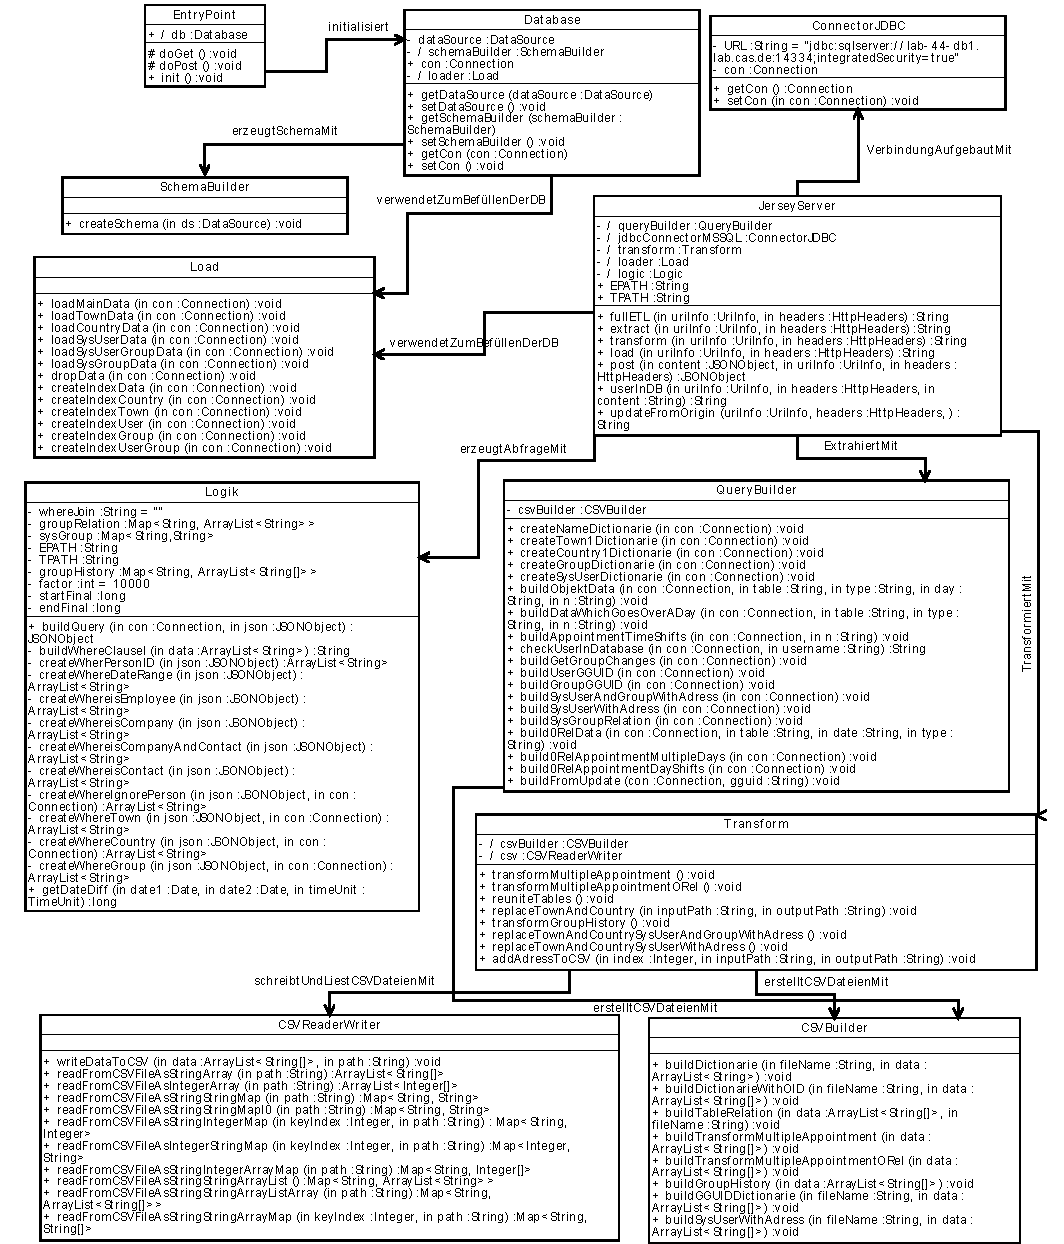
\includegraphics[width=1.0\textwidth]{pics/ServerKlassendiagramm.pdf}
\caption{Server Klassendiagramm}
\label{umsetzung_klassendiagramm_server}
\end{center}
\end{figure}

%% ===========================
\section{Klassen des Clients}
%% ===========================

\begin{figure}[htbp]
\begin{center}
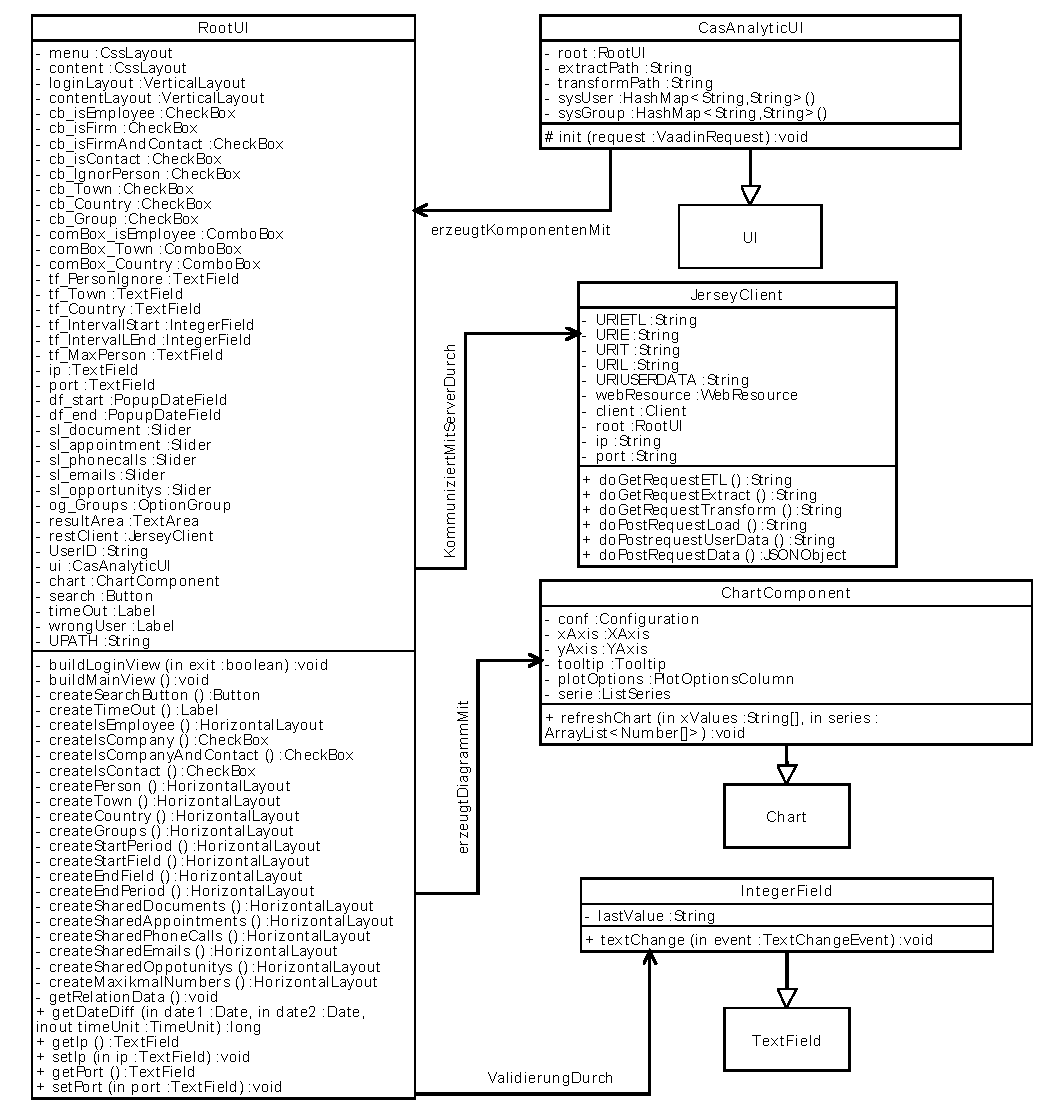
\includegraphics[width=1.0\textwidth]{pics/ClientKlassendiagramm.pdf}
\caption{Client Klassendiagramm}
\label{umsetzung_klassendiagramm_client}
\end{center}
\end{figure}